\documentclass[11pt,letterpaper]{article}
\usepackage[margin=0.8in,top=0.85in,bottom=0.8in]{geometry}
\usepackage[T1]{fontenc}
\usepackage[utf8]{inputenc}
\usepackage{newtxtext,newtxmath,microtype,graphicx,booktabs,longtable,array,tabularx,multirow,xcolor,fancyhdr,lastpage,pdflscape,caption,tocloft,hyperref,colortbl}
\hypersetup{colorlinks=true,linkcolor=black,urlcolor=blue,pdftitle=Reserve Management Plan}
\definecolor{linegray}{HTML}{C8CDD2}
\definecolor{sectionblue}{HTML}{3A5F7D}
\definecolor{softgray}{HTML}{F6F7F8}
\setlength{\headheight}{16pt}
\pagestyle{fancy}
\fancyhf{}
\fancyhead[L]{\footnotesize Ridge Park Luxury Condominiums Owners' Association Inc.}
\fancyhead[R]{\footnotesize January 1, 2026}
\fancyfoot[L]{\footnotesize Reserve Study Report}
\fancyfoot[R]{\footnotesize Page \thepage\ of \pageref{LastPage}}
\setlength{\parindent}{0pt}
\setlength{\parskip}{0.45em}
\renewcommand{\arraystretch}{1.18}

\newcommand{\sectionrule}{\par\vspace{0.2em}{\color{linegray}\rule{\linewidth}{0.6pt}}\par\vspace{0.6em}}
\newcommand{\reportsection}[1]{%
  \par\vspace{0.2em}%
  \addcontentsline{toc}{section}{#1}%
  {{\Large\bfseries\color{sectionblue} #1\par}}%
  \sectionrule
}
\newcommand{\subnote}[1]{\vspace{0.3em}\colorbox{softgray}{\parbox{0.97\linewidth}{\small #1}}\vspace{0.4em}}

\begin{document}

\thispagestyle{empty}
\begin{flushleft}
{\small Board of Directors}\\
{\small Ridge Park Luxury Condominiums Owners' Association Inc.}\\
{\small Los Alamos, New Mexico}
\end{flushleft}

\vspace{0.8em}
Please find the attached report on the current Ridge Park reserve study.  This study was compiled using project schedules discussed by the Maintenance and the Budget Committe in a joint meeting on April 22, 2026. The purpose of this report is to provide an idea of the overall mainenance needs and schedules anticipated over the next 30 years to ensure the common elements are maintained in good condition, thereby keeping the community safe, preserving home values, and ensuring a positive living experience in the community.

The report is intended to mirror the structure and feel of a conventional reserve study.  The purpose is not to replace a proefsional reserve study, but to provide a transparent and digestable format.

The reserve model remains a planning tool rather than a prediction of exact future outcomes. Actual repair timing, pricing, inflation, and investment returns will differ from the assumptions used here. The goal is to keep the association approximately funded at approximately the right time and to make both short- and long-range reserve decisions easier to review.

Sincerely,\\[0.7em]
Brendan J. Gifford\\
Ridge Park Treasurer
\newpage

\thispagestyle{empty}
\begin{center}
\vspace*{1.2cm}
{\LARGE\bfseries Ridge Park Luxury Condominiums Owners' Association Inc.}\\[2.0cm]
{\Huge\bfseries Reserve Management Plan}\\[0.45cm]
{\Large\bfseries Type 1}\\[0.45cm]
{\LARGE\bfseries Reserve Study with Data-Driven Analysis}\\[1.7cm]
{\large\bfseries For 30-Year Projection Period Beginning January 1, 2026}\\[1.0cm]
\IfFileExists{cover_img.png}{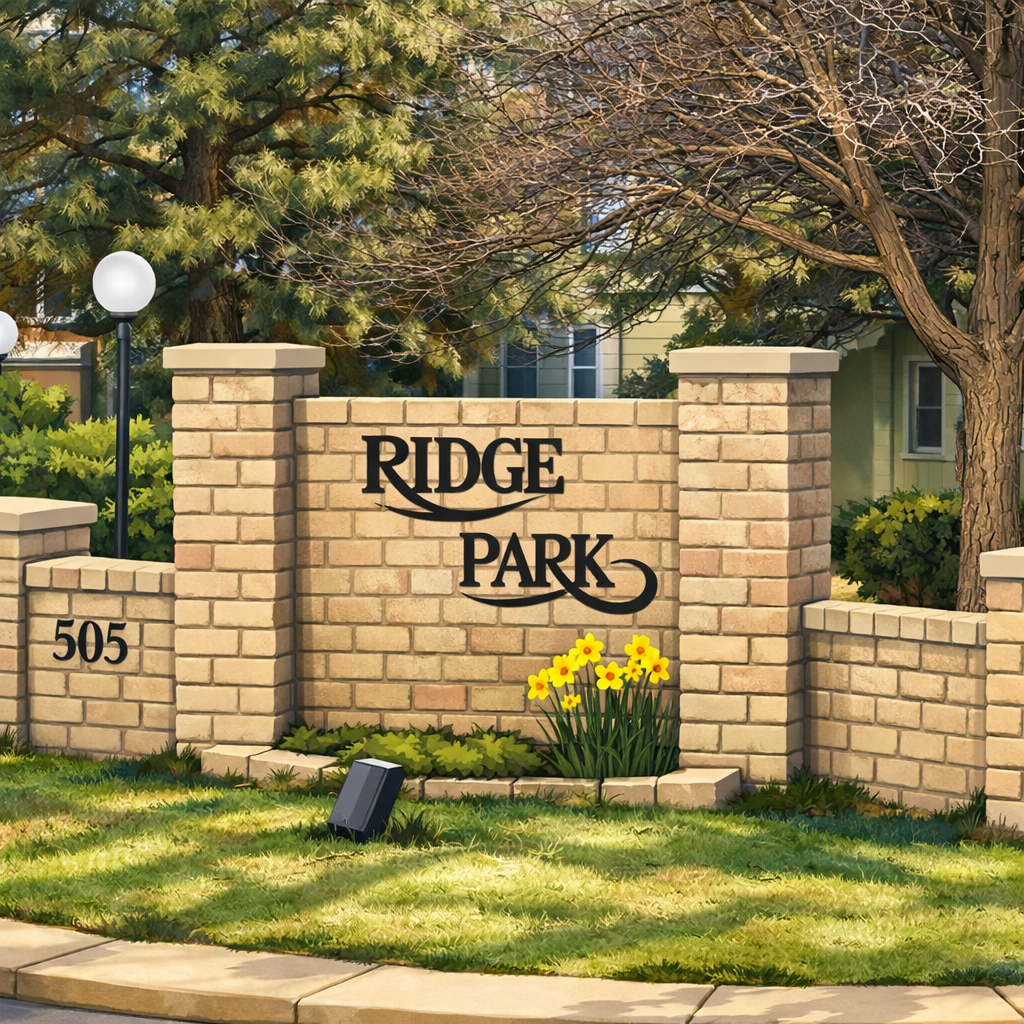
\includegraphics[width=0.68\linewidth]{cover_img.png}}{\vspace{3cm}}
\end{center}
\newpage

\tableofcontents
\newpage

\reportsection{Preparer's Report on Reserve Study}
{\bfseries Report Description}\\
This report was generated using a custom-built Python package. The workflow reads the Association’s reserve assumptions, component inventory, replacement schedule, annual contribution plan, and reserve cash-flow projection, then produces a report in the format of a typical reserve study.

The report is intended to serve as a planning tool and to establish a baseline for future revisions as the Association’s long-term reserve priorities, project scopes, and funding needs become clearer.

The assessment requirements shown in this report were generated with short-term affordability in mind. The objectives were to begin with an assessment level generally consistent with what homeowners are paying in 2026, increase assessments over the first five years sufficiently to address major deferred-maintenance projects expected during that period, and maintain sufficient reserve funding for longer-term projects. These include, among other items, roofing repairs, pavement repairs, siding replacement, and related exterior-building needs.

{\bfseries Engagement between Maintenance and Budget Committees}\\
The Ridge Park Maintenance and Budget Committees met on April 15, 2026, to discuss maintenance priorities for 2026 and beyond. The committees reviewed maintenance schedules and estimates from the 2024 Reserve Plan. As a result of that discussion, the following components were introduced, revised, or rescheduled within the reserve study.

Unless otherwise stated, the dollar figures discussed in this section are shown in current dollars and are not adjusted for inflation. Inflation adjustments are incorporated in the maintenance schedules underlying the overall reserve study.

a. The structural engineering report identified the need to install railings around the patio area adjacent to the pool. The Maintenance Committee obtained estimates for this work, totaling approximately \$21,000, and this amount has been integrated into the 2026 work plan.

b. The committees discussed the scope of the chimney chase structural renovations originally identified in the 2024 Reserve Study. This component has been broken into an annual cost beginning in the current year and continuing over the next six years. The estimate assumes that 23 chimney chases will be repaired each year at a cost of \$2,500 per chase, for a total of \$57,500 per year over the next six years. This component is then scheduled to recur every 20 years.

c. Asphalt crack repair is scheduled for 2026 at an estimated cost of \$50,000. This work is expected to recur in four years. Approximately nine years from now, the plan shifts to a mill-and-overlay project covering approximately 100,000 square feet of asphalt.

d. The original reserve study included \$8,000 per year for tree and shrub trimming, and that recurring amount is maintained in this version. Because the 2025 Board budgeted \$15,000 for this item, an additional one-time expense of \$7,000 has been added in 2026. This allows the reserve plan to reflect a \$15,000 expenditure in 2026 without disrupting the recurring long-term funding assumption.

e. The 2026 plan includes \$25,000 for gutter repairs to continue the work begun last year. The model then assumes that \$25,000 will be spent every five years, which is approximately equivalent to collecting \$5,000 per year for this component.

f. Buildings 2, 3, 4, 6, and 7 are scheduled for repainting in 2026 at a cost of \$3 per square foot, for a total estimated cost of \$185,000. The model assumes these buildings will be repainted again in 10 years. The remaining buildings are scheduled for repainting over the following two years and follow the same recurring schedule.

g. The original 2024 Reserve Study called for replacement of all building siding beginning immediately. The joint committee agreed that this schedule is likely too aggressive given the estimated \$1.5 million cost. The committee also noted that the siding replacements associated with the repainting of Building 5 last year were satisfactory and were included in the painting price. However, that may not be the case when other buildings are repainted. This reserve study therefore schedules full siding replacement to align with the next paint cycle, beginning in 2035 and continuing through 2037.

h. Metal stairway flashing and stringer repairs are included at \$15,000 to cover work associated with multiple stairwells. This item is then scheduled to recur every seven years. Additional review may be needed to ensure that the remaining maintenance schedule is sufficiently funded.

i. Skylight replacement has been included at \$5,000. Because this item was not included in the original reserve study, further research should be conducted to determine whether it should be treated as a recurring reserve component.

j. Fascia, flashing, and soffit repairs were included in the 2024 Reserve Study, but only at \$10,000 every eight years, beginning in 2026. To ensure anticipated 2026 expenditures are covered, an additional \$55,000 has been added in 2026.

k. Balcony, deck, and structural-support work is included beginning in 2027. The model assumes 23 repairs per year at \$2,500 each, for a total of \$57,500 per year, continuing through 2031. This component is then scheduled to recur every 20 years.

l. Replacement of one or two dumpster surrounds is scheduled for 2026 at a total estimated cost of \$7,500. A design plan should be developed before this work proceeds.

m. Concrete work on the grouted walls was originally scheduled every three years at a cost of \$2,500. The Maintenance Committee has identified an additional \$12,000 of work it would like to complete in 2026. This amount has been added as a one-time cost so the recurring contribution schedule can be preserved.

n. Total landscape work of \$13,500 is planned for 2026. This includes wildfire defensible-space planning, border blocks, and landscape replenishment.

o. Parking lot restriping in the amount of \$5,000 is included in the 2026 plan.

p. Several smaller inspection and maintenance items are included in the plan. These include roof inspection and repair (\$17,000), water valve inspection (\$1,800), sewer inspection (\$5,000), and lateral sewer-line cleanout (\$5,000). These items begin in 2026 and recur every other year.

q. The brick wall beside the pool requires repair estimated at \$2,500, which is budgeted in 2026. This item recurs at the same rate as other brick-wall components on the property.

{\bfseries Management’s Responsibility}\\
Management remains responsible for the assumptions underlying the reserve model. These include inflation, investment return, beginning reserve balance, component scope, useful-life estimates, replacement timing, and any planned contribution or special-assessment strategy.

The Board and committees should review all assumptions and estimates for accuracy, completeness, and reasonableness. The preparer may lack the technical expertise, project-specific knowledge, or operational insight needed to independently verify all maintenance assumptions and cost estimates.

{\bfseries Preparer Responsibility}\\
The preparer’s responsibility is limited to organizing the supplied data into financial exhibits, narrative disclosures, and summary schedules. The preparer is also responsible for ensuring that the report-generation process, data handling, and algorithms used by the custom Python package function as intended.

The preparer does not independently certify the accuracy of the underlying maintenance estimates, engineering assumptions, useful-life determinations, or Board-approved funding strategy.

{\bfseries Important Limitations}\\
This report should be read together with the full set of assumptions, source data, schedules, and component-level details underlying the reserve model.

If any underlying source data changes, including component costs, project timing, useful-life assumptions, beginning balances, contribution schedules, inflation assumptions, or investment-return assumptions, the report should be regenerated so that the tables, exhibits, and summary metrics remain aligned with the current model.

\subnote{This document was not prepared by a credentialed professional. It is best treated as a transparent analytical report, not as a substitute for a professional reserve study.}

\newpage
\reportsection{Statement of Position}
\begin{tabularx}{\linewidth}{>{\bfseries}l X}
Projection period: & 2026 to 2055 \\
Type of project: & Reserve Study \\
Number of units: & 138 \\
Location: & Los Alamos, New Mexico \\
Project construction date: & 1984 \\
Analysis date: & January 1, 2026 \\
Report prepared by: & Brendan J. Gifford, Treasurer \\
\end{tabularx}

\vspace{0.8em}
\begin{tabularx}{\linewidth}{X r}
\toprule
Metric & Value \\
\midrule
\rowcolor{blue!12} Current Replacement Cost & \$6,252,328 \\
Future Replacement Cost & \$9,038,538 \\
\rowcolor{blue!12} Current Reserve Fund Balance & \$620,000 \\
Fully Funded Reserve Balance & \$3,208,492 \\
\rowcolor{blue!12} Percent Funded & 19.32 \% \\
Reserve Deficit & \$2,588,492 \\
\rowcolor{blue!12} Reserve Deficit per Unit & \$18,757 \\
Projected Annual Reserve Contribution & \$250,000 \\
\rowcolor{blue!12} Average Annual Reserve Contribution per Unit & \$1,812 \\
Projected Monthly Reserve Contribution & \$20,833 \\
\rowcolor{blue!12} Average Monthly Reserve Contribution per Unit & \$151 \\
\bottomrule
\end{tabularx}

\subnote{First-year reserve contribution: \$250,000. First-year ending balance: \$281,597. Ending balance in the final projection year (2055): \$5,820,418.}

\newpage
\reportsection{Summary of Major Components}
{\small Analysis Date - January 1, 2026 \quad Inflation: 3.00\% \quad Investment: 2.50\% \quad Contribution Factor: 0.00}

\vspace{0.6em}
\begin{tabularx}{\linewidth}{X >{\centering\arraybackslash}p{1.3cm} >{\centering\arraybackslash}p{2.2cm} >{\centering\arraybackslash}p{2.3cm} >{\raggedleft\arraybackslash}p{2.7cm}}
\toprule
Category & Useful Lives & Replacement Years & Remaining Years & Future Cost \\
\midrule
\rowcolor{blue!12} Exterior Surfaces & 7-30 & 2026-2045 & 0:06-19:06 & \$2,917,769 \\
Roofing & 2-30 & 2026-2040 & 0:06-14:06 & \$2,602,459 \\
\rowcolor{blue!12} Asphalt & 3-30 & 2026-2056 & 0:06-30:06 & \$2,097,660 \\
Painting & 3-12 & 2026-2036 & 0:06-10:06 & \$582,014 \\
\rowcolor{blue!12} Balconies-Decks-Stairways & 5-30 & 2026-2031 & 0:06-5:06 & \$451,767 \\
Flooring & 12-20 & 2034 & 8:06 & \$75,081 \\
\rowcolor{blue!12} Renovation & 10-20 & 2029-2039 & 3:06-13:06 & \$63,913 \\
Doors-Windows & 10-30 & 2026-2036 & 0:06-10:06 & \$53,460 \\
\rowcolor{blue!12} Concrete & 3-25 & 2026-2044 & 0:06-18:06 & \$48,231 \\
Fences-Walls-Gates & 3-25 & 2026-2036 & 0:06-10:06 & \$47,645 \\
\rowcolor{blue!12} Landscape & 1-8 & 2026-2031 & 0:06-5:06 & \$31,866 \\
Equipment & 7-25 & 2028-2036 & 2:06-10:06 & \$29,002 \\
\rowcolor{blue!12} Plumbing & 2-12 & 2026-2031 & 0:06-5:06 & \$13,838 \\
Structural & 5-10 & 2026-2028 & 0:06-2:06 & \$12,995 \\
\rowcolor{blue!12} Fire Safety & 5 & 2029 & 3:06 & \$5,545 \\
Signage & 5-20 & 2026-2029 & 0:06-3:06 & \$5,292 \\
\bottomrule
\end{tabularx}

\newpage
\reportsection{Percent Funded - Annual - Ending Balance}
\begin{longtable}{>{\centering\arraybackslash}p{1.4cm} >{\raggedleft\arraybackslash}p{2.6cm} >{\raggedleft\arraybackslash}p{2.7cm} >{\raggedleft\arraybackslash}p{2.0cm}}
\toprule
Year & Ending Balance & Funded Balance & Percent Funded \\
\midrule
\endfirsthead
\toprule
Year & Ending Balance & Funded Balance & Percent Funded \\
\midrule
\endhead
\rowcolor{blue!12} 2026 & \$281,597 & \$3,040,186 & 9.26\% \\
2027 & \$332,715 & \$3,224,469 & 10.32\% \\
\rowcolor{blue!12} 2028 & \$364,793 & \$3,358,136 & 10.86\% \\
2029 & \$572,165 & \$3,631,243 & 15.76\% \\
\rowcolor{blue!12} 2030 & \$830,292 & \$3,913,935 & 21.21\% \\
2031 & \$970,181 & \$4,035,531 & 24.04\% \\
\rowcolor{blue!12} 2032 & \$1,453,725 & \$4,493,835 & 32.35\% \\
2033 & \$1,891,729 & \$4,899,674 & 38.61\% \\
\rowcolor{blue!12} 2034 & \$2,323,061 & \$5,292,034 & 43.90\% \\
2035 & \$2,268,276 & \$5,186,660 & 43.73\% \\
\rowcolor{blue!12} 2036 & \$1,502,456 & \$4,355,278 & 34.50\% \\
2037 & \$1,343,816 & \$4,131,587 & 32.53\% \\
\rowcolor{blue!12} 2038 & \$1,100,527 & \$3,823,940 & 28.78\% \\
2039 & \$1,025,616 & \$3,686,520 & 27.82\% \\
\rowcolor{blue!12} 2040 & \$939,479 & \$3,540,199 & 26.54\% \\
2041 & \$1,213,095 & \$3,758,040 & 32.28\% \\
\rowcolor{blue!12} 2042 & \$1,589,653 & \$4,084,353 & 38.92\% \\
2043 & \$1,944,739 & \$4,395,288 & 44.25\% \\
\rowcolor{blue!12} 2044 & \$2,218,989 & \$4,630,797 & 47.92\% \\
2045 & \$2,508,403 & \$4,870,739 & 51.50\% \\
\rowcolor{blue!12} 2046 & \$1,966,063 & \$4,263,691 & 46.11\% \\
2047 & \$2,168,179 & \$4,395,580 & 49.33\% \\
\rowcolor{blue!12} 2048 & \$2,350,557 & \$4,501,997 & 52.21\% \\
2049 & \$2,908,642 & \$4,979,720 & 58.41\% \\
\rowcolor{blue!12} 2050 & \$3,314,241 & \$5,299,701 & 62.54\% \\
2051 & \$3,599,618 & \$5,501,970 & 65.42\% \\
\rowcolor{blue!12} 2052 & \$4,222,848 & \$6,046,502 & 69.84\% \\
2053 & \$4,727,992 & \$6,468,284 & 73.09\% \\
\rowcolor{blue!12} 2054 & \$5,217,614 & \$6,869,508 & 75.95\% \\
2055 & \$5,820,418 & \$7,379,078 & 78.88\% \\
\bottomrule
\end{longtable}

\newpage
\reportsection{Cash Flow - Annual}
\begin{longtable}{>{\centering\arraybackslash}p{1.1cm} >{\raggedleft\arraybackslash}p{2.0cm} >{\raggedleft\arraybackslash}p{1.9cm} >{\raggedleft\arraybackslash}p{2.1cm} >{\raggedleft\arraybackslash}p{1.9cm} >{\raggedleft\arraybackslash}p{1.7cm} >{\raggedleft\arraybackslash}p{2.0cm}}
\toprule
Year & Begin & Contribution & Special Assess. & Expenditures & Interest & Ending \\
\midrule
\endfirsthead
\toprule
Year & Begin & Contribution & Special Assess. & Expenditures & Interest & Ending \\
\midrule
\endhead
\rowcolor{blue!12} 2026 & \$620,000 & \$250,000 & \$0 & \$601,204 & \$12,802 & \$281,597 \\
2027 & \$281,597 & \$300,000 & \$0 & \$257,405 & \$8,522 & \$332,715 \\
\rowcolor{blue!12} 2028 & \$332,715 & \$350,000 & \$0 & \$327,685 & \$9,762 & \$364,793 \\
2029 & \$364,793 & \$400,000 & \$0 & \$205,164 & \$12,537 & \$572,165 \\
\rowcolor{blue!12} 2030 & \$572,165 & \$450,000 & \$0 & \$210,283 & \$18,410 & \$830,292 \\
2031 & \$830,292 & \$500,000 & \$0 & \$383,915 & \$23,804 & \$970,181 \\
\rowcolor{blue!12} 2032 & \$970,181 & \$520,000 & \$0 & \$67,381 & \$30,925 & \$1,453,725 \\
2033 & \$1,453,725 & \$540,000 & \$0 & \$144,615 & \$42,618 & \$1,891,729 \\
\rowcolor{blue!12} 2034 & \$1,891,729 & \$560,000 & \$0 & \$182,242 & \$53,574 & \$2,323,061 \\
2035 & \$2,323,061 & \$580,000 & \$0 & \$694,184 & \$59,400 & \$2,268,276 \\
\rowcolor{blue!12} 2036 & \$2,268,276 & \$600,000 & \$0 & \$1,416,552 & \$50,731 & \$1,502,456 \\
2037 & \$1,502,456 & \$610,000 & \$0 & \$806,522 & \$37,882 & \$1,343,816 \\
\rowcolor{blue!12} 2038 & \$1,343,816 & \$620,000 & \$0 & \$896,356 & \$33,067 & \$1,100,527 \\
2039 & \$1,100,527 & \$630,000 & \$0 & \$733,664 & \$28,753 & \$1,025,616 \\
\rowcolor{blue!12} 2040 & \$1,025,616 & \$640,000 & \$0 & \$752,930 & \$26,794 & \$939,479 \\
2041 & \$939,479 & \$650,000 & \$0 & \$404,778 & \$28,394 & \$1,213,095 \\
\rowcolor{blue!12} 2042 & \$1,213,095 & \$660,000 & \$0 & \$319,780 & \$36,338 & \$1,589,653 \\
2043 & \$1,589,653 & \$670,000 & \$0 & \$360,486 & \$45,572 & \$1,944,739 \\
\rowcolor{blue!12} 2044 & \$1,944,739 & \$680,973 & \$0 & \$460,379 & \$53,656 & \$2,218,989 \\
2045 & \$2,218,989 & \$701,402 & \$0 & \$472,730 & \$60,741 & \$2,508,403 \\
\rowcolor{blue!12} 2046 & \$2,508,403 & \$722,444 & \$0 & \$1,324,223 & \$59,440 & \$1,966,063 \\
2047 & \$1,966,063 & \$744,118 & \$0 & \$595,645 & \$53,642 & \$2,168,179 \\
\rowcolor{blue!12} 2048 & \$2,168,179 & \$766,441 & \$0 & \$642,629 & \$58,566 & \$2,350,557 \\
2049 & \$2,350,557 & \$789,435 & \$0 & \$298,443 & \$67,093 & \$2,908,642 \\
\rowcolor{blue!12} 2050 & \$2,908,642 & \$813,118 & \$0 & \$487,074 & \$79,556 & \$3,314,241 \\
2051 & \$3,314,241 & \$837,511 & \$0 & \$640,673 & \$88,539 & \$3,599,618 \\
\rowcolor{blue!12} 2052 & \$3,599,618 & \$862,637 & \$0 & \$338,664 & \$99,258 & \$4,222,848 \\
2053 & \$4,222,848 & \$888,516 & \$0 & \$497,087 & \$113,714 & \$4,727,992 \\
\rowcolor{blue!12} 2054 & \$4,727,992 & \$915,171 & \$0 & \$551,829 & \$126,280 & \$5,217,614 \\
2055 & \$5,217,614 & \$942,626 & \$0 & \$479,612 & \$139,791 & \$5,820,418 \\
\bottomrule
\end{longtable}

\newpage
\reportsection{Disclosures}
\begin{itemize}
\item This report was generated from current component inventory and condition, projected expenditures, annual contribution schedules, and reserve cash-flow projections.
\item Analysis date: January 1, 2026. Projection horizon: 30 years.
\item Inflation assumption used in the model: 3.00\%.
\item Investment return assumption used in the model: 2.50\%.
\item Beginning reserve balance used in the projection: \$620,000.
\item While component replacement timing and cost estimates are best guesses, actual field conditions may cause different timing or scope.
\item This document is formatted to resemble a conventional reserve study using custom Python-based software designed and written by Brendan J. Gifford rather than from proprietary reserve-study software.
\item Readers should review contribution levels, projected expenditures, and percent-funded results together. No single table should be interpreted in isolation.
\end{itemize}

\newpage
\begin{landscape}
\reportsection{Expenditures Matrix: Years 1--10}
\scriptsize
\setlength{\tabcolsep}{4.0pt}
\begin{tabular}{p{4.2cm}*{10}{r}}
\toprule
Category & 2026 & 2027 & 2028 & 2029 & 2030 & 2031 & 2032 & 2033 & 2034 & 2035 \\
\midrule
\rowcolor{blue!12} Asphalt & \$50,744 &  &  &  & \$28,557 &  &  &  &  & \$397,260 \\
Balconies-Decks-Stairways & \$102,504 & \$60,107 & \$92,058 & \$63,767 & \$65,680 & \$67,651 &  & \$49,927 & \$9,642 &  \\
\rowcolor{blue!12} Concrete & \$15,223 &  &  & \$16,635 &  &  & \$18,177 &  &  & \$19,863 \\
Doors-Windows & \$6,089 &  &  &  &  &  &  &  &  & \$22,820 \\
\rowcolor{blue!12} Equipment &  &  & \$6,331 &  & \$1,713 & \$3,000 & \$909 &  &  &  \\
Exterior Surfaces & \$124,324 & \$60,107 & \$61,910 & \$74,857 & \$65,680 & \$173,539 &  & \$6,241 & \$12,856 &  \\
\rowcolor{blue!12} Fences-Walls-Gates & \$17,253 &  & \$1,615 & \$11,090 &  & \$2,941 & \$3,030 & \$1,872 & \$6,428 & \$3,310 \\
Fire Safety &  &  &  & \$5,545 &  &  &  &  & \$6,428 &  \\
\rowcolor{blue!12} Flooring &  &  &  &  &  &  &  &  & \$75,081 &  \\
Landscape & \$28,924 & \$18,816 & \$19,381 & \$23,843 & \$20,561 & \$24,119 & \$26,054 & \$22,467 & \$23,141 & \$28,470 \\
\rowcolor{blue!12} Painting & \$192,860 & \$118,375 & \$127,169 & \$5,545 & \$15,695 &  & \$6,059 &  & \$3,857 & \$82,943 \\
Plumbing & \$11,015 &  & \$11,685 &  & \$12,397 & \$2,824 & \$13,152 &  & \$13,953 &  \\
\rowcolor{blue!12} Renovation &  &  &  & \$2,772 &  & \$8,824 &  &  & \$30,855 &  \\
Roofing & \$42,625 &  &  &  &  & \$89,840 &  & \$64,107 &  & \$139,518 \\
\rowcolor{blue!12} Signage & \$2,030 &  & \$2,153 & \$1,109 &  & \$2,353 &  &  &  &  \\
Structural & \$7,612 &  & \$5,383 &  &  & \$8,824 &  &  &  &  \\
\bottomrule
\end{tabular}
\end{landscape}

\newpage
\begin{landscape}
\reportsection{Expenditures Matrix: Years 11--20}
\scriptsize
\setlength{\tabcolsep}{4.0pt}
\begin{tabular}{p{4.2cm}*{10}{r}}
\toprule
Category & 2036 & 2037 & 2038 & 2039 & 2040 & 2041 & 2042 & 2043 & 2044 & 2045 \\
\midrule
\rowcolor{blue!12} Asphalt &  &  & \$36,175 &  & \$61,404 & \$39,529 &  &  & \$43,195 & \$71,185 \\
Balconies-Decks-Stairways & \$4,092 &  & \$36,175 &  & \$23,027 &  & \$12,214 & \$41,936 & \$5,183 &  \\
\rowcolor{blue!12} Concrete &  &  & \$21,705 &  &  & \$23,717 &  &  & \$58,924 &  \\
Doors-Windows & \$24,551 &  &  &  &  &  &  &  &  &  \\
\rowcolor{blue!12} Equipment & \$17,049 & \$2,107 &  &  & \$4,421 &  &  & \$5,032 & \$2,592 &  \\
Exterior Surfaces & \$223,957 & \$210,727 & \$217,048 & \$223,560 & \$230,267 & \$237,175 & \$260,576 & \$276,780 & \$259,167 & \$266,942 \\
\rowcolor{blue!12} Fences-Walls-Gates & \$23,869 &  & \$5,788 & \$11,178 &  & \$7,906 &  & \$2,516 & \$12,958 &  \\
Fire Safety &  &  &  & \$7,452 &  &  &  &  & \$8,639 &  \\
\rowcolor{blue!12} Flooring &  &  &  &  &  &  &  &  &  &  \\
Landscape & \$24,551 & \$25,287 & \$31,110 & \$30,553 & \$27,632 & \$33,995 & \$29,315 & \$30,194 & \$37,147 & \$32,033 \\
\rowcolor{blue!12} Painting & \$300,106 & \$159,086 & \$178,139 &  & \$21,092 & \$7,906 &  &  & \$13,822 & \$102,570 \\
Plumbing & \$14,803 &  & \$15,704 &  & \$16,661 &  & \$17,675 & \$4,026 & \$18,752 &  \\
\rowcolor{blue!12} Renovation &  &  &  & \$25,188 &  &  &  &  &  &  \\
Roofing & \$770,618 & \$409,315 & \$347,277 & \$434,243 & \$368,427 & \$39,529 &  &  &  &  \\
\rowcolor{blue!12} Signage & \$2,728 &  &  & \$1,490 &  & \$3,162 &  &  &  &  \\
Structural & \$10,229 &  & \$7,235 &  &  & \$11,859 &  &  &  &  \\
\bottomrule
\end{tabular}
\end{landscape}

\newpage
\begin{landscape}
\reportsection{Expenditures Matrix: Years 21--30}
\scriptsize
\setlength{\tabcolsep}{4.0pt}
\begin{tabular}{p{4.2cm}*{10}{r}}
\toprule
Category & 2046 & 2047 & 2048 & 2049 & 2050 & 2051 & 2052 & 2053 & 2054 & 2055 \\
\midrule
\rowcolor{blue!12} Asphalt &  & \$47,200 &  &  & \$51,577 & \$254,994 & \$262,644 & \$326,883 & \$278,639 & \$286,998 \\
Balconies-Decks-Stairways & \$105,398 & \$136,879 & \$160,432 & \$115,171 & \$134,099 & \$122,185 & \$6,566 & \$56,359 & \$34,830 &  \\
\rowcolor{blue!12} Concrete &  & \$28,320 &  &  & \$30,946 &  &  & \$33,815 &  &  \\
Doors-Windows & \$32,994 &  &  &  &  &  &  &  &  &  \\
\rowcolor{blue!12} Equipment & \$4,674 & \$1,416 &  &  &  & \$8,500 & \$6,303 &  &  &  \\
Exterior Surfaces & \$105,398 & \$108,560 & \$111,816 & \$115,171 & \$159,887 & \$122,185 &  & \$11,272 &  &  \\
\rowcolor{blue!12} Fences-Walls-Gates & \$4,583 & \$4,720 & \$2,917 & \$15,022 & \$5,158 & \$5,312 &  & \$9,017 & \$11,610 &  \\
Fire Safety &  &  &  & \$10,015 &  &  &  &  & \$11,610 &  \\
\rowcolor{blue!12} Flooring & \$65,988 &  &  &  &  &  &  &  & \$52,013 &  \\
Landscape & \$32,994 & \$45,312 & \$35,003 & \$36,053 & \$44,356 & \$38,249 & \$39,397 & \$48,469 & \$41,796 & \$49,029 \\
\rowcolor{blue!12} Painting & \$339,162 & \$223,238 & \$297,743 &  & \$38,662 &  &  & \$11,272 & \$6,966 & \$137,845 \\
Plumbing & \$19,894 &  & \$21,105 &  & \$22,390 &  & \$23,754 &  & \$25,201 & \$5,740 \\
\rowcolor{blue!12} Renovation &  &  &  & \$5,007 &  & \$15,937 &  &  & \$89,165 &  \\
Roofing & \$595,726 &  &  &  &  & \$53,124 &  &  &  &  \\
\rowcolor{blue!12} Signage & \$3,666 &  & \$3,889 & \$2,003 &  & \$4,250 &  &  &  &  \\
Structural & \$13,748 &  & \$9,723 &  &  & \$15,937 &  &  &  &  \\
\bottomrule
\end{tabular}
\end{landscape}

\newpage
\reportsection{Component List - Summary}
\scriptsize
\begin{longtable}{p{4.2cm} p{1.6cm} r r r c c r}
\toprule
\textbf{Category} & \textbf{Replace} & \textbf{Basis Cost} & \textbf{Quantity} & \textbf{Current Cost} & \textbf{Est Life} & \textbf{Rem Life} & \textbf{Future Cost} \\
\textbf{Component} & \textbf{Date} &  &  &  &  &  &  \\
\midrule
\endfirsthead
\toprule
\textbf{Category} & \textbf{Replace} & \textbf{Basis Cost} & \textbf{Quantity} & \textbf{Current Cost} & \textbf{Est Life} & \textbf{Rem Life} & \textbf{Future Cost} \\
\textbf{Component} & \textbf{Date} &  &  &  &  &  &  \\
\midrule
\endhead
\multicolumn{8}{l}{\textbf{Asphalt}} \\
\rowcolor{blue!12} Asphalt Crack Seal & 7/26 - 7/38 & \$50,000 & 3 & \$100,000 & 3 & 0:06-12:06 & \$115,476 \\
Asphalt Mill and Overlay & 7/35 - 7/35 & \$3 & 100,000 & \$300,000 & 15 & 9:06 & \$397,260 \\
\rowcolor{blue!12} Asphalt Seal Coat & 7/40 - 7/56 & \$0 & 300,000 & \$120,000 & 5 & 14:06-30:06 & \$231,125 \\
Asphalt Remove and Replace & 7/51 - 7/55 & \$6 & 100,000 & \$600,000 & 30 & 25:06-29:06 & \$1,353,799 \\
\addlinespace[1pt] \multicolumn{4}{r}{} & \textbf{\$1,120,000} & & & \textbf{\$2,097,660} \\
\addlinespace[6pt]
\multicolumn{8}{l}{\textbf{Balconies-Decks-Stairways}} \\
\rowcolor{blue!12} Adding Walkway Railing & 7/26 & \$21,000 & 1 & \$21,000 & 30 & 0:06 & \$21,313 \\
Metal Stairway Flashing/Stringers & 7/26 & \$15,000 & 1 & \$15,000 & 7 & 0:06 & \$15,223 \\
\rowcolor{blue!12} Stairway/Balcony Railing & 7/26 - 7/26 & \$7,500 & 24 & \$65,000 & 8-20 & 0:06 & \$65,968 \\
Balconies-Decks-Posts/Structural Supports & 7/27 - 7/31 & \$2,500 & 115 & \$287,500 & 20 & 1:06-5:06 & \$319,115 \\
\rowcolor{blue!12} Walkway Railing & 7/28 & \$3,000 & 1 & \$3,000 & 8 & 2:06 & \$3,230 \\
Wood Balcony Walls & 7/28 & \$25,000 & 1 & \$25,000 & 5 & 2:06 & \$26,917 \\
\addlinespace[1pt] \multicolumn{4}{r}{} & \textbf{\$416,500} & & & \textbf{\$451,767} \\
\addlinespace[6pt]
\multicolumn{8}{l}{\textbf{Concrete}} \\
\rowcolor{blue!12} Concrete Sidewalks-Stairs-Patios/Grinding-Repairs & 7/26 & \$10,000 & 1 & \$10,000 & 3 & 0:06 & \$10,149 \\
Curbs-Gutters & 7/26 & \$5,000 & 1 & \$5,000 & 3 & 0:06 & \$5,074 \\
\rowcolor{blue!12} Pool Area Concrete Deck & 7/44 & \$12 & 1,592 & \$19,104 & 25 & 18:06 & \$33,008 \\
\addlinespace[1pt] \multicolumn{4}{r}{} & \textbf{\$34,104} & & & \textbf{\$48,231} \\
\addlinespace[6pt]
\multicolumn{8}{l}{\textbf{Doors-Windows}} \\
Skylights & 7/26 & \$6,000 & 1 & \$6,000 & 30 & 0:06 & \$6,089 \\
\rowcolor{blue!12} Raise and Replace Windows & 7/35 & \$17,233 & 1 & \$17,233 & 30 & 9:06 & \$22,820 \\
Clubhouse Bathroom/Interior Doors & 7/36 & \$5,000 & 1 & \$5,000 & 10 & 10:06 & \$6,820 \\
\rowcolor{blue!12} Clubhouse Blinds & 7/36 & \$1,000 & 1 & \$1,000 & 10 & 10:06 & \$1,364 \\
Clubhouse Glass Doors & 7/36 & \$3,500 & 1 & \$3,500 & 10 & 10:06 & \$4,774 \\
\rowcolor{blue!12} Clubhouse Sliding Glass Doors & 7/36 & \$4,000 & 1 & \$4,000 & 10 & 10:06 & \$5,456 \\
Clubhouse/Fitness Windows & 7/36 & \$4,500 & 1 & \$4,500 & 10 & 10:06 & \$6,138 \\
\addlinespace[1pt] \multicolumn{4}{r}{} & \textbf{\$41,233} & & & \textbf{\$53,460} \\
\addlinespace[6pt]
\multicolumn{8}{l}{\textbf{Equipment}} \\
\rowcolor{blue!12} Pool Cover & 7/28 & \$4 & 720 & \$2,880 & 12 & 2:06 & \$3,101 \\
Pool Heater Raypak & 7/28 & \$3,000 & 1 & \$3,000 & 15 & 2:06 & \$3,230 \\
\rowcolor{blue!12} Pool Misc Pipes Valves & 7/30 & \$1,500 & 1 & \$1,500 & 7 & 4:06 & \$1,713 \\
Pool Filter Hayward & 7/31 & \$1,300 & 1 & \$1,300 & 15 & 5:06 & \$1,530 \\
\rowcolor{blue!12} Pool Rails-Ladder & 7/31 & \$250 & 3 & \$750 & 15 & 5:06 & \$882 \\
Pool Room Compressor & 7/31 & \$500 & 1 & \$500 & 15 & 5:06 & \$588 \\
\rowcolor{blue!12} Pool Pump Hayward & 7/32 & \$750 & 1 & \$750 & 15 & 6:06 & \$909 \\
Mail Boxes & 7/36 & \$10,000 & 1 & \$10,000 & 25 & 10:06 & \$13,639 \\
\rowcolor{blue!12} Pool Chemical Controller-Rola Chem & 7/36 & \$2,500 & 1 & \$2,500 & 15 & 10:06 & \$3,410 \\
\addlinespace[1pt] \multicolumn{4}{r}{} & \textbf{\$23,180} & & & \textbf{\$29,002} \\
\addlinespace[6pt]
\multicolumn{8}{l}{\textbf{Exterior Surfaces}} \\
Chimney Chases Structural Renovations & 7/26 - 7/31 & \$2,500 & 138 & \$345,000 & 20 & 0:06-5:06 & \$377,471 \\
\rowcolor{blue!12} Fascia-Flashing-Soffits & 7/26 - 7/26 & \$55,000 & 2 & \$65,000 & 8 & 0:06 & \$65,968 \\
Stucco Siding Repair & 7/29 & \$10,000 & 1 & \$10,000 & 7 & 3:06 & \$11,090 \\
\rowcolor{blue!12} Clubhouse Siding & 7/31 & \$12 & 7,500 & \$90,000 & 30 & 5:06 & \$105,888 \\
Corrugated Balcony Walls & 7/33 & \$5,000 & 1 & \$5,000 & 10 & 7:06 & \$6,241 \\
\rowcolor{blue!12} Pool Coping & 7/36 & \$35 & 120 & \$4,200 & 20 & 10:06 & \$5,728 \\
Wood Siding & 7/36 - 7/45 & \$12 & 125,000 & \$1,500,000 & 30 & 10:06-19:06 & \$2,345,383 \\
\addlinespace[1pt] \multicolumn{4}{r}{} & \textbf{\$2,019,200} & & & \textbf{\$2,917,769} \\
\addlinespace[6pt]
\multicolumn{8}{l}{\textbf{Fences-Walls-Gates}} \\
\rowcolor{blue!12} Concrete Brick Grouted Wall & 7/26 - 7/26 & \$12,000 & 2 & \$14,500 & 3 & 0:06 & \$14,716 \\
Pool Area Wall Repair & 7/26 & \$2,500 & 1 & \$2,500 & 5 & 0:06 & \$2,537 \\
\rowcolor{blue!12} Stacked Concrete Block Wall & 7/28 & \$1,500 & 1 & \$1,500 & 5 & 2:06 & \$1,615 \\
Chain Link Fence & 7/29 & \$2,500 & 1 & \$2,500 & 10 & 3:06 & \$2,772 \\
\rowcolor{blue!12} Wooden Perimeter Fence & 7/29 & \$5,000 & 1 & \$5,000 & 5 & 3:06 & \$5,545 \\
Pool Area Metal Rail Fence-Gate & 7/36 & \$75 & 200 & \$15,000 & 25 & 10:06 & \$20,459 \\
\addlinespace[1pt] \multicolumn{4}{r}{} & \textbf{\$41,000} & & & \textbf{\$47,645} \\
\addlinespace[6pt]
\multicolumn{8}{l}{\textbf{Fire Safety}} \\
\rowcolor{blue!12} Chimney Flues-Caps-Spark Arrestors & 7/29 & \$5,000 & 1 & \$5,000 & 5 & 3:06 & \$5,545 \\
\addlinespace[1pt] \multicolumn{4}{r}{} & \textbf{\$5,000} & & & \textbf{\$5,545} \\
\addlinespace[6pt]
\multicolumn{8}{l}{\textbf{Flooring}} \\
Clubhouse Carpet & 7/34 & \$9 & 4,000 & \$36,000 & 12 & 8:06 & \$46,283 \\
\rowcolor{blue!12} Clubhouse Tile Floor & 7/34 & \$16 & 1,000 & \$16,000 & 20 & 8:06 & \$20,570 \\
Pool Area Tile Exterior & 7/34 & \$16 & 400 & \$6,400 & 20 & 8:06 & \$8,228 \\
\addlinespace[1pt] \multicolumn{4}{r}{} & \textbf{\$58,400} & & & \textbf{\$75,081} \\
\addlinespace[6pt]
\multicolumn{8}{l}{\textbf{Landscape}} \\
\rowcolor{blue!12} Landscape Border Blocks & 7/26 & \$1,000 & 1 & \$1,000 & 3 & 0:06 & \$1,015 \\
Landscape Replenishment & 7/26 & \$2,500 & 1 & \$2,500 & 3 & 0:06 & \$2,537 \\
\rowcolor{blue!12} Landscaping, Wildfire Defensible Space & 7/26 & \$10,000 & 1 & \$10,000 & 1 & 0:06 & \$10,149 \\
Tree Removal-Major Trimming & 7/26 - 7/26 & \$8,000 & 2 & \$15,000 & 1 & 0:06 & \$15,223 \\
\rowcolor{blue!12} Landscape Rock & 7/31 & \$2,500 & 1 & \$2,500 & 8 & 5:06 & \$2,941 \\
\addlinespace[1pt] \multicolumn{4}{r}{} & \textbf{\$31,000} & & & \textbf{\$31,866} \\
\addlinespace[6pt]
\multicolumn{8}{l}{\textbf{Painting}} \\
Painting Building 2 & 7/26 & \$3 & 11,539 & \$34,617 & 10 & 0:06 & \$35,132 \\
\rowcolor{blue!12} Painting Building 3 & 7/26 & \$3 & 11,213 & \$33,639 & 10 & 0:06 & \$34,140 \\
Painting Building 4 & 7/26 & \$3 & 15,029 & \$45,087 & 10 & 0:06 & \$45,758 \\
\rowcolor{blue!12} Painting Building 6 & 7/26 & \$3 & 11,948 & \$35,844 & 10 & 0:06 & \$36,378 \\
Painting Building 7 & 7/26 & \$3 & 11,948 & \$35,844 & 10 & 0:06 & \$36,378 \\
\rowcolor{blue!12} Parking Striping-Curb Painting & 7/26 & \$5,000 & 1 & \$5,000 & 3 & 0:06 & \$5,074 \\
Painting Building 1 & 7/27 & \$3 & 11,539 & \$34,617 & 10 & 1:06 & \$36,186 \\
\rowcolor{blue!12} Painting Building 13 & 7/27 & \$3 & 11,799 & \$35,397 & 10 & 1:06 & \$37,002 \\
Painting Building 8 & 7/27 & \$3 & 14,409 & \$43,227 & 10 & 1:06 & \$45,187 \\
\rowcolor{blue!12} Painting Building 10 & 7/28 & \$3 & 11,799 & \$35,397 & 10 & 2:06 & \$38,112 \\
Painting Building 11 & 7/28 & \$3 & 7,886 & \$23,658 & 10 & 2:06 & \$25,472 \\
\rowcolor{blue!12} Painting Building 12 & 7/28 & \$3 & 11,799 & \$35,397 & 10 & 2:06 & \$38,112 \\
Painting Building 9 & 7/28 & \$3 & 7,886 & \$23,658 & 10 & 2:06 & \$25,472 \\
\rowcolor{blue!12} Painting Buidling 14 & 7/30 & \$3 & 4,580 & \$13,740 & 10 & 4:06 & \$15,695 \\
Pool Area Metal Rail Fence-Gate-Painting & 7/34 & \$15 & 200 & \$3,000 & 10 & 8:06 & \$3,857 \\
\rowcolor{blue!12} Painting Building 5 & 7/35 & \$4 & 14,409 & \$57,636 & 10 & 9:06 & \$76,322 \\
Clubhouse Interior Painting & 7/36 & \$2 & 20,000 & \$35,000 & 12 & 10:06 & \$47,737 \\
\addlinespace[1pt] \multicolumn{4}{r}{} & \textbf{\$530,758} & & & \textbf{\$582,014} \\
\addlinespace[6pt]
\multicolumn{8}{l}{\textbf{Plumbing}} \\
\rowcolor{blue!12} Sewer Inspection, Semi-annual Inspection & 7/26 & \$4,097 & 1 & \$4,097 & 2 & 0:06 & \$4,158 \\
Sewer Lateral Lines-Cleanouts & 7/26 & \$5,000 & 1 & \$5,000 & 2 & 0:06 & \$5,074 \\
\rowcolor{blue!12} Water Valve and Line Annual Inspection & 7/26 & \$1,756 & 1 & \$1,756 & 2 & 0:06 & \$1,782 \\
Clubhouse Hot Water Heaters-Expansion & 7/31 & \$1,200 & 2 & \$2,400 & 12 & 5:06 & \$2,824 \\
\addlinespace[1pt] \multicolumn{4}{r}{} & \textbf{\$13,253} & & & \textbf{\$13,838} \\
\addlinespace[6pt]
\multicolumn{8}{l}{\textbf{Renovation}} \\
\rowcolor{blue!12} Clubhouse Maintenance Shop Remodel & 7/29 & \$2,500 & 1 & \$2,500 & 10 & 3:06 & \$2,772 \\
Clubhouse Pool Room-Shower Remodel & 7/31 & \$5,000 & 1 & \$5,000 & 20 & 5:06 & \$5,883 \\
\rowcolor{blue!12} Sauna Remodel & 7/31 & \$2,500 & 1 & \$2,500 & 20 & 5:06 & \$2,941 \\
Clubhouse Bar Remodel & 7/34 & \$5,000 & 1 & \$5,000 & 20 & 8:06 & \$6,428 \\
\rowcolor{blue!12} Clubhouse Bathroom Remodel & 7/34 & \$6,000 & 2 & \$12,000 & 20 & 8:06 & \$15,428 \\
Fitness Room Kitchenette Remodel & 7/34 & \$3,500 & 1 & \$3,500 & 20 & 8:06 & \$4,500 \\
\rowcolor{blue!12} Laundry Room Remodel & 7/34 & \$3,500 & 1 & \$3,500 & 20 & 8:06 & \$4,500 \\
Pool Resurface & 7/39 & \$12 & 1,200 & \$14,400 & 15 & 13:06 & \$21,462 \\
\addlinespace[1pt] \multicolumn{4}{r}{} & \textbf{\$48,400} & & & \textbf{\$63,913} \\
\addlinespace[6pt]
\multicolumn{8}{l}{\textbf{Roofing}} \\
\rowcolor{blue!12} Gutters-Downspouts & 7/26 & \$25,000 & 1 & \$25,000 & 5 & 0:06 & \$25,372 \\
Roof Inspection and Repair & 7/26 & \$17,000 & 1 & \$17,000 & 2 & 0:06 & \$17,253 \\
\rowcolor{blue!12} Carport Roofs & 7/31 - 7/39 & \$12 & 21,400 & \$256,800 & 25 & 5:06-13:06 & \$341,244 \\
Clubhouse Roof & 7/35 & \$12 & 4,500 & \$54,000 & 25 & 9:06 & \$71,507 \\
\rowcolor{blue!12} Garage Flat Roof & 7/36 & \$300,000 & 1 & \$300,000 & 10 & 10:06 & \$409,178 \\
Unit Building Shingle Roofs & 7/36 - 7/40 & \$12 & 100,000 & \$1,200,000 & 30 & 10:06-14:06 & \$1,737,905 \\
\addlinespace[1pt] \multicolumn{4}{r}{} & \textbf{\$1,852,800} & & & \textbf{\$2,602,459} \\
\addlinespace[6pt]
\multicolumn{8}{l}{\textbf{Signage}} \\
\rowcolor{blue!12} Building Signs/Numbers & 7/26 & \$2,000 & 1 & \$2,000 & 5 & 0:06 & \$2,030 \\
Monument Sign/Wall & 7/28 & \$2,000 & 1 & \$2,000 & 20 & 2:06 & \$2,153 \\
\rowcolor{blue!12} Misc and Parking Signs & 7/29 & \$1,000 & 1 & \$1,000 & 10 & 3:06 & \$1,109 \\
\addlinespace[1pt] \multicolumn{4}{r}{} & \textbf{\$5,000} & & & \textbf{\$5,292} \\
\addlinespace[6pt]
\multicolumn{8}{l}{\textbf{Structural}} \\
Trash Enclosures & 7/26 & \$7,500 & 1 & \$7,500 & 5 & 0:06 & \$7,612 \\
\rowcolor{blue!12} Carport Support Posts-Beams & 7/28 & \$5,000 & 1 & \$5,000 & 10 & 2:06 & \$5,383 \\
\addlinespace[1pt] \multicolumn{4}{r}{} & \textbf{\$12,500} & & & \textbf{\$12,995} \\
\addlinespace[6pt]
\bottomrule
\end{longtable}

\newpage
\reportsection{Upcoming Major Components}
\begin{longtable}{>{\centering\arraybackslash}p{2.0cm} p{2.6cm} p{7.0cm} >{\raggedleft\arraybackslash}p{2.3cm}}
\toprule
Date & Category & Component & Future Cost \\
\midrule
\endfirsthead
\toprule
Date & Category & Component & Future Cost \\
\midrule
\endhead
\rowcolor{blue!12} 2026-07-01 & Balconies-Decks-Stairways & Stairway/Balcony Railing & \$58,356 \\
2026-07-01 & Exterior Surfaces & Chimney Chases Structural Renovations & \$58,356 \\
\rowcolor{blue!12} 2026-07-01 & Exterior Surfaces & Fascia-Flashing-Soffits & \$55,819 \\
2026-07-01 & Asphalt & Asphalt Crack Seal & \$50,744 \\
\rowcolor{blue!12} 2026-07-01 & Painting & Painting Building 4 & \$45,758 \\
2026-07-01 & Painting & Painting Building 6 & \$36,378 \\
\rowcolor{blue!12} 2026-07-01 & Painting & Painting Building 7 & \$36,378 \\
2026-07-01 & Painting & Painting Building 2 & \$35,132 \\
\rowcolor{blue!12} 2026-07-01 & Painting & Painting Building 3 & \$34,140 \\
2026-07-01 & Roofing & Gutters-Downspouts & \$25,372 \\
\rowcolor{blue!12} 2026-07-01 & Balconies-Decks-Stairways & Adding Walkway Railing & \$21,313 \\
2026-07-01 & Roofing & Roof Inspection and Repair & \$17,253 \\
\rowcolor{blue!12} 2026-07-01 & Balconies-Decks-Stairways & Metal Stairway Flashing/Stringers & \$15,223 \\
2026-07-01 & Fences-Walls-Gates & Concrete Brick Grouted Wall & \$12,179 \\
\rowcolor{blue!12} 2026-07-01 & Concrete & Concrete Sidewalks-Stairs-Patios/Grinding-Repairs & \$10,149 \\
2026-07-01 & Exterior Surfaces & Fascia-Flashing-Soffits & \$10,149 \\
\rowcolor{blue!12} 2026-07-01 & Landscape & Landscaping, Wildfire Defensible Space & \$10,149 \\
2026-07-01 & Landscape & Tree Removal-Major Trimming & \$8,119 \\
\bottomrule
\end{longtable}

\subnote{Largest summarized category by future cost: Exterior Surfaces at \$2,917,769. Lowest year-end reserve balance in the projection occurs in 2026, at \$281,597. Highest projected percent funded occurs in 2055, at 78.88\%.}

\end{document}
